\section{Experimental and Theoretical Setup}

\begin{frame}{The ALICE Experiment at the LHC}
\begin{figure}[H]
\centering
\includegraphics[width = 0.6\textwidth]{figures/alice}
\caption{Schematic picture of the ALICE detector at the LHC at CERN in Geneva.\footnotemark \\
The experiment is specialized on heavy-ion collisions (mostly Pb-Pb) and reaches center-of-mass energies of $\sqrt{s} = 5.02\ \mathrm{TeV}$.}	
\end{figure}
\footnotetext{Figure taken from ALICEinfo: \tiny{\url{http://aliceinfo.cern.ch/Public/en/Chapter2/Chap2Experiment-en.html} (26.06.2020)}}
\end{frame}

\begin{frame}{The RHIC at the Brookhaven National Lab}
\begin{figure}[H]
\centering
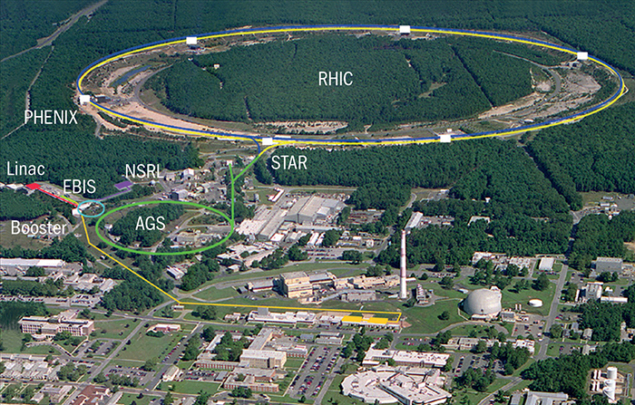
\includegraphics[width = 0.6\textwidth]{figures/rhic_overview}
\caption{The RHIC at the Brookhaven National Lab.\footnotemark \\ The different experiments (STAR, sPHENIX\footnotemark) study different aspects of the QGP and the spin structure of the proton. Center-of-mass energies of $\sqrt{s} = 500\ \mathrm{GeV}$ are reached.}	
\end{figure}
\footnotetext[2]{Figure taken from CernCourier: \tiny{\url{https://cerncourier.com/a/rhics-new-gold-record/} (26.06.2020)}\vspace{0.5em}}
\footnotetext{Replaces PHENIX (operated until 2016). Preliminary starts operating in 2023.}
\end{frame}

\begin{frame}{The Situation immediately after the Collision I}
\vspace{0.5em}
\alert{Question}: How do the partons freed by a RHIC thermalize?\\[0.5em]

\begin{itemize}
	\item The thermalization process provides a starting point for \alert{hydrodynamical evolution} in terms of the \alert{energy-momentum tensor} $T^{\mu\nu}$.
	\item The dominant parton contribution is dominated by \alert{gluon saturation} and occupation numbers $\sim 1/\alpha_s$.
	\item Theoretical model: \alert{Color-Glass condensate} effective field theory (CQC).
\end{itemize}
\begin{figure}
	\centering
	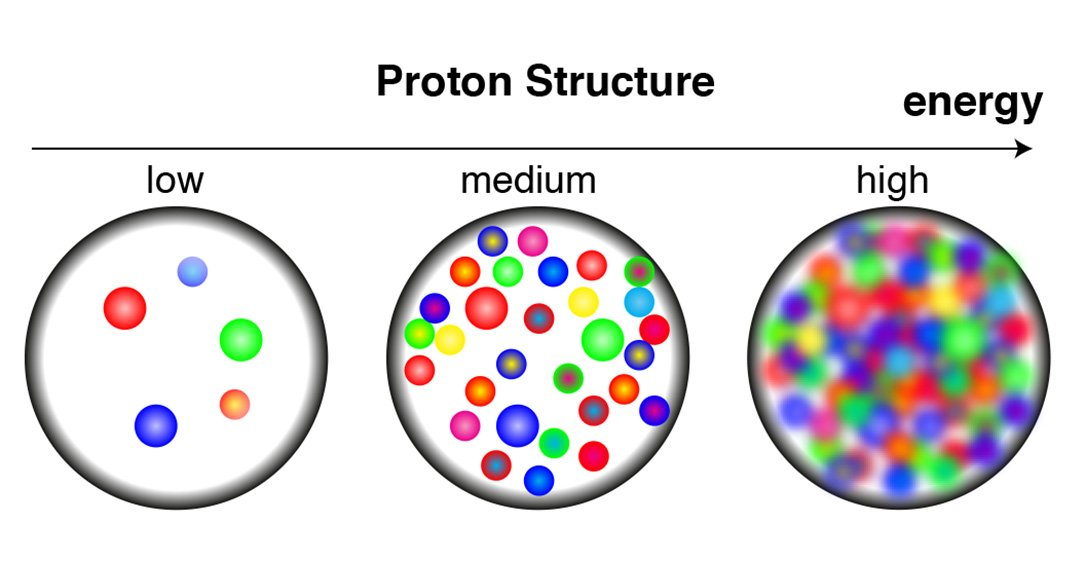
\includegraphics[width=0.5\textwidth]{figures/cqc}
	\caption{Visualization of the Color-Glass Condensate model.\footnotemark}
\end{figure}
\footnote{Source: \tiny\url{https://www.uu.nl/en/research/institute-for-subatomic-physics/research/color-glass-condensate} (29.06.2020)}
\end{frame}

\begin{frame}{The Situation immediately after the Collision II}
\begin{itemize}
	\item \alert{Problem:} The initial situation $T^{\phantom{.}\mu\nu}_{\mathrm{Glasma}} = \operatorname{diag}(\varepsilon,\varepsilon,\varepsilon,-\varepsilon)$, does \alert{not} serve as starting point!
	\item \alert{Expectation:} Situation changes rapidly on a time scale $\sim 1/Q_{\mathrm{s}}$.
\end{itemize}
\vspace{0.5em}	
But does the phase-space distribution function relax towards the expected equilibrium \alert{Bose-Einstein distribution}?\\[0.5em]
\begin{itemize}
	\item \alert{Bottom-Up approach:} Relaxation as a result of hard elastic and inelastic collisions. 
\end{itemize}
\end{frame}

\begin{frame}{The overpopulated Quark-Gluon-Plasma}
The following discussion is based on the publications \cite{Blaizot2012} and \cite{Blaizot2016}.\\[0.5em]
\begin{itemize}
	\item Typical gluon energy densities: $\varepsilon_0 = \varepsilon(\tau=Q_{\mathrm{s}}^{-1})\sim \frac{Q_{\mathrm{s}}^{4}}{\alpha_{\mathrm{s}}}$
	\item Gluons produced per unit volume: $n_0 = n(\tau=Q_{\mathrm{s}}^{-1})\sim \frac{Q_{\mathrm{s}}^{3}}{\alpha_{\mathrm{s}}}$
	\item This implies that the average energy per gluon is $\varepsilon_0/n_0 \sim Q_{\mathrm{s}}$.	
\end{itemize}
\vspace{0.5em}
Comparison with the equilibrated system at temperature $T$ leaves a mismatch:\\[0.5em]
\begin{itemize}
	\item Assume an initial distribution of the form $n_0\cdot\varepsilon_0^{-3/4}\sim 1/\alpha_{\mathrm{s}}^{1/4}$.
	\item In equilibrium we know $\varepsilon_{\mathrm{eq}} \sim T^{\phantom{.}4}$, $n_{\mathrm{eq}} \sim T^{\phantom{.}3}$ and $n_{\mathrm{eq}}\cdot\varepsilon_{\mathrm{eq}}^{-3/4}\sim 1$.
\end{itemize}
\vspace{0.5em}
Mismatch by a \alert{large} factor of $\alpha_{\mathrm{s}}^{-1/4}$ corresponding to an \alert{overpopulation} of the initial distribution. \ ($\alpha_{\mathrm{s}} \ll 1 $ in weak coupling asymptotics)
\end{frame}

